\documentclass{standalone}
\usepackage{tikz-network}
\begin{document}
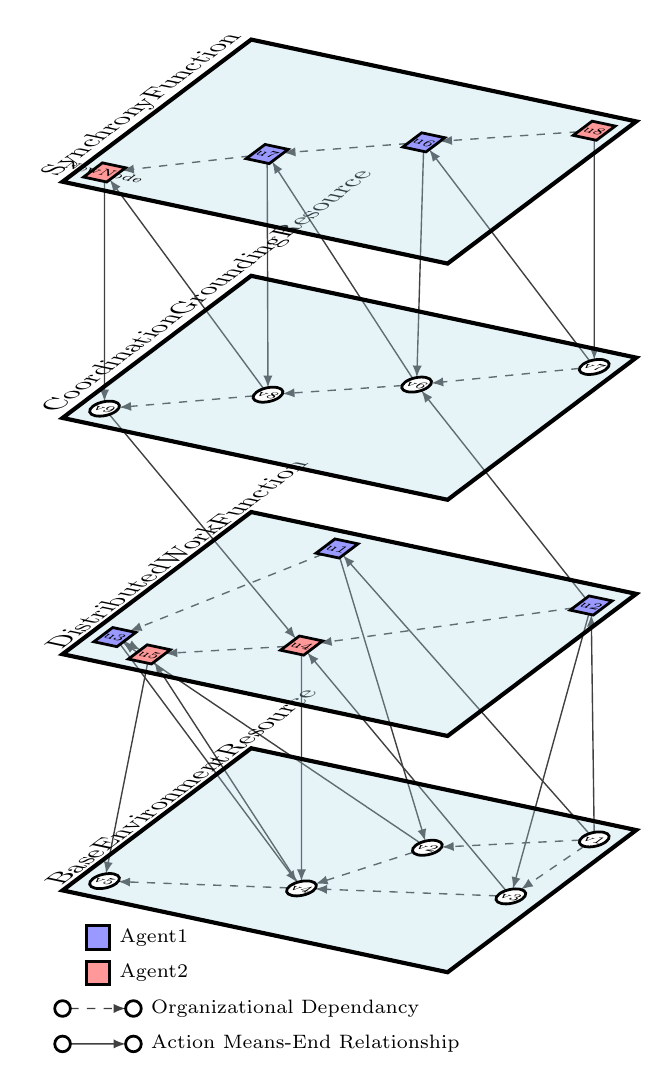
\begin{tikzpicture}[multilayer=3d]
\SetPlaneWidth{5}
\SetPlaneHeight{3}
\SetLayerDistance{-3}
\SetVertexStyle[FillColor=white]\Plane[layer=4]
\Text[layer=4,position=above right,rotation=90]{BaseEnvironmentResource}
\Plane[layer=3]
\Text[layer=3,position=above right,rotation=90]{DistributedWorkFunction}
\Plane[layer=2]
\Text[layer=2,position=above right,rotation=90]{CoordinationGroundingResource}
\Plane[layer=1]
\Text[layer=1,position=above right,rotation=90]{SynchronyFunction}
\Vertex[x=4.7,y=2.7,size=0.3,label=v1,fontsize=\tiny,layer=4,]{v1}
\Vertex[x=3.122,y=1.978,size=0.3,label=v2,fontsize=\tiny,layer=4,]{v2}
\Vertex[x=4.621,y=1.47,size=0.3,label=v3,fontsize=\tiny,layer=4,]{v3}
\Vertex[x=2.393,y=0.869,size=0.3,label=v4,fontsize=\tiny,layer=4,]{v4}
\Vertex[x=0.3,y=0.3,size=0.3,label=v5,fontsize=\tiny,layer=4,]{v5}
\Vertex[x=3.138,y=1.788,size=0.3,label=v6,fontsize=\tiny,layer=2,]{v6}
\Vertex[x=4.7,y=2.7,size=0.3,label=v7,fontsize=\tiny,layer=2,]{v7}
\Vertex[x=1.768,y=1.102,size=0.3,label=v8,fontsize=\tiny,layer=2,]{v8}
\Vertex[x=0.3,y=0.3,size=0.3,label=v9,fontsize=\tiny,layer=2,]{v9}
\Vertex[x=1.36,y=2.7,size=0.3,label=u1,fontsize=\tiny,layer=3,shape=rectangle,RGB,color={153,153,255}]{u1}
\Vertex[x=4.7,y=2.651,size=0.3,label=u2,fontsize=\tiny,layer=3,shape=rectangle,RGB,color={153,153,255}]{u2}
\Vertex[x=0.3,y=0.464,size=0.3,label=u3,fontsize=\tiny,layer=3,shape=rectangle,RGB,color={153,153,255}]{u3}
\Vertex[x=2.305,y=0.978,size=0.3,label=u4,fontsize=\tiny,layer=3,shape=rectangle,RGB,color={255,153,153}]{u4}
\Vertex[x=0.882,y=0.3,size=0.3,label=u5,fontsize=\tiny,layer=3,shape=rectangle,RGB,color={255,153,153}]{u5}
\Vertex[x=3.13,y=1.912,size=0.3,label=u6,fontsize=\tiny,layer=1,shape=rectangle,RGB,color={153,153,255}]{u6}
\Vertex[x=1.7,y=1.172,size=0.3,label=u7,fontsize=\tiny,layer=1,shape=rectangle,RGB,color={153,153,255}]{u7}
\Vertex[x=4.7,y=2.7,size=0.3,label=u8,fontsize=\tiny,layer=1,shape=rectangle,RGB,color={255,153,153}]{u8}
\Vertex[x=0.3,y=0.3,size=0.3,label=NewNode,fontsize=\tiny,layer=1,shape=rectangle,RGB,color={255,153,153}]{NewNode}
\Edge[Direct,lw=0.5pt,style={dashed}](v1)(v2)
\Edge[Direct,lw=0.5pt,style={dashed}](v1)(v3)
\Edge[Direct,lw=0.5pt](v1)(u1)
\Edge[Direct,lw=0.5pt](v1)(u2)
\Edge[Direct,lw=0.5pt,style={dashed}](v2)(v4)
\Edge[Direct,lw=0.5pt](v2)(u3)
\Edge[Direct,lw=0.5pt,style={dashed}](v3)(v4)
\Edge[Direct,lw=0.5pt](v3)(u4)
\Edge[Direct,lw=0.5pt,style={dashed}](v4)(v5)
\Edge[Direct,lw=0.5pt](v4)(u5)
\Edge[Direct,lw=0.5pt,style={dashed}](v6)(v8)
\Edge[Direct,lw=0.5pt](v6)(u7)
\Edge[Direct,lw=0.5pt,style={dashed}](v7)(v6)
\Edge[Direct,lw=0.5pt](v7)(u6)
\Edge[Direct,lw=0.5pt,style={dashed}](v8)(v9)
\Edge[Direct,lw=0.5pt](v8)(NewNode)
\Edge[Direct,lw=0.5pt](v9)(u4)
\Edge[Direct,lw=0.5pt](u1)(v2)
\Edge[Direct,lw=0.5pt,style={dashed}](u1)(u3)
\Edge[Direct,lw=0.5pt](u2)(v3)
\Edge[Direct,lw=0.5pt,style={dashed}](u2)(u4)
\Edge[Direct,lw=0.5pt](u2)(v6)
\Edge[Direct,lw=0.5pt](u3)(v4)
\Edge[Direct,lw=0.5pt,style={dashed}](u3)(u5)
\Edge[Direct,lw=0.5pt](u4)(v4)
\Edge[Direct,lw=0.5pt,style={dashed}](u4)(u5)
\Edge[Direct,lw=0.5pt](u5)(v5)
\Edge[Direct,lw=0.5pt](u6)(v6)
\Edge[Direct,lw=0.5pt,style={dashed}](u6)(u7)
\Edge[Direct,lw=0.5pt](u7)(v8)
\Edge[Direct,lw=0.5pt,style={dashed}](u7)(NewNode)
\Edge[Direct,lw=0.5pt](u8)(v7)
\Edge[Direct,lw=0.5pt,style={dashed}](u8)(u6)
\Edge[Direct,lw=0.5pt](NewNode)(v9)
\Vertex[x=0.45,y=-9.6,size=0.3,shape=rectangle,RGB,color={153,153,255},label=Agent1,position=0]{agent1}
\Vertex[x=0.45,y=-10.05,size=0.3,shape=rectangle,RGB,color={255,153,153},label=Agent2,position=0]{agent2}
\Vertex[x=0,y=-10.5,size=0]{e11}
\Vertex[x=0.9,y=-10.5,size=0,label=Organizational Dependancy,position=0]{e12}
\Edge[Direct,lw=0.5pt,style={dashed}](e11)(e12)
\Vertex[x=0,y=-10.95,size=0]{e21}
\Vertex[x=0.9,y=-10.95,size=0,label=Action Means-End Relationship,position=0]{e22}
\Edge[Direct,lw=0.5pt](e21)(e22)
\end{tikzpicture}
\end{document}
